\documentclass{article}
\usepackage[utf8]{inputenc}
\usepackage{amsmath}
\usepackage{amssymb}
\usepackage{amsthm}
\usepackage{float}
\usepackage[colorlinks=true]{hyperref}
\usepackage{parskip}
\usepackage{ upgreek }
\usepackage{tikz}
\usetikzlibrary{arrows,automata}
\usepackage{fancyhdr}
\usepackage[a4paper, total={6in, 8in}]{geometry}




\pagestyle{fancy}
\lhead{1. Endelige tilstandsautomater}
\rhead{Elsie Mestl}

\title{INF1820\\Oblig 1b}
\date{\today}
\author{Elsie Mestl}

\setcounter{secnumdepth}{0}

\begin{document}
\subsection{1.}
$\mathcal{L}_1 = \{w \,|\, w \text{ ikke inneholder substingen }bab \}$

Begynner å lage en DFA som akksepterer kun strenger som inneholder substrengern $''bab''$

\begin{center}
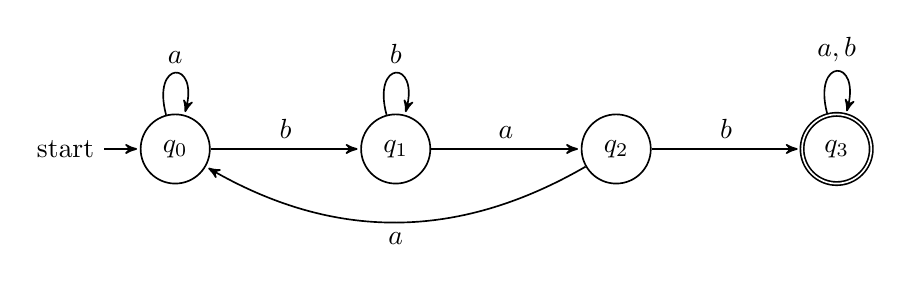
\begin{tikzpicture}[->,>=stealth',shorten >=1pt,auto,node distance=2.8cm,
    semithick]
  \node[initial, state] (q01) {$q_0$};
  \node[state] (q11) [right of=q01] {$q_1$};
  \node[state] (q21) [right of=q11] {$q_2$};
  \node[state, accepting] (q31) [right of=q21] {$q_3$};
  \path (q01) edge node {$b$} (q11)
  edge [loop above] node {$a$} (q01)
  (q11) edge [loop above] node {$b$} (q11)
  edge node {$a$} (q21)
  (q21) edge [bend left] node {$a$} (q01)
  edge node {$b$} (q31)
  (q31) edge [loop above] node {$a, b$} (q31);
\end{tikzpicture}
\end{center}

Det inverterte av tilstandsmaskinen over er den tilstandsmaskinen vi leter etter. Alle trenger som IKKE inneholder substrengern $''bab''$ og siden det er en DFA vet vi at for å invertere holder det å flippe alle statsene til accepting hvis de ikke er det eller non-accepting hvis de originalt var det. Og vi får:

\begin{center}
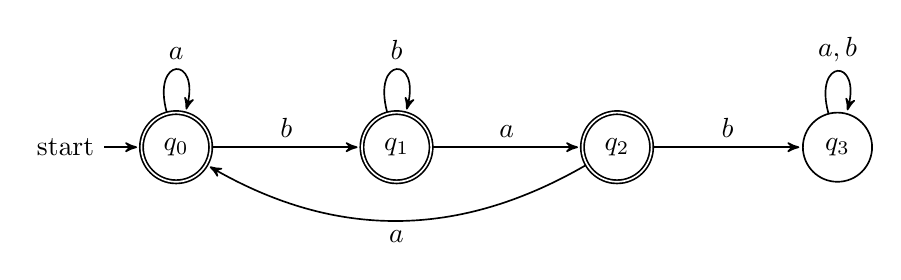
\begin{tikzpicture}[->,>=stealth',shorten >=1pt,auto,node distance=2.8cm,
    semithick]
  \node[initial, state, accepting] (q01) {$q_0$};
  \node[state, accepting] (q11) [right of=q01] {$q_1$};
  \node[state, accepting] (q21) [right of=q11] {$q_2$};
  \node[state] (q31) [right of=q21] {$q_3$};
  \path (q01) edge node {$b$} (q11)
  edge [loop above] node {$a$} (q01)
  (q11) edge [loop above] node {$b$} (q11)
  edge node {$a$} (q21)
  (q21) edge [bend left] node {$a$} (q01)
  edge node {$b$} (q31)
  (q31) edge [loop above] node {$a, b$} (q31);
\end{tikzpicture}
\end{center}

\subsection{2.}
$\mathcal{L}_2 = \{w \,|\, w \text{ inneholder substringen }aa \}$

\begin{center}
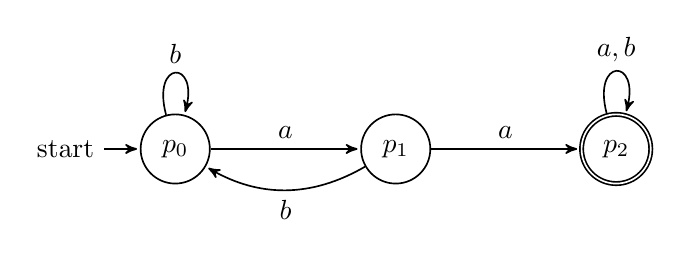
\begin{tikzpicture}[->,>=stealth',shorten >=1pt,auto,node distance=2.8cm,
    semithick]
  \node[initial, state] (q02) {$p_0$};
  \node[state] (q12) [right of=q02] {$p_1$};
  \node[state, accepting] (q22) [right of=q12] {$p_2$};
  \path (q02) edge node {$a$} (q12)
  edge [loop above] node {$b$} (q02)
  (q12) edge [bend left] node {$b$} (q02)
  edge node {$a$} (q22)
  (q22) edge [loop above] node {$a, b$} (q22);
\end{tikzpicture}
\end{center}

Ikke så mye forklaring som trengs her.

\newpage

\subsection{3.}
$\mathcal{L}_3 = \mathcal{L}_1 \cup \mathcal{L}_2$

Begynner med å lage en NFA som accepterer $\mathcal{L}_3$

\begin{center}
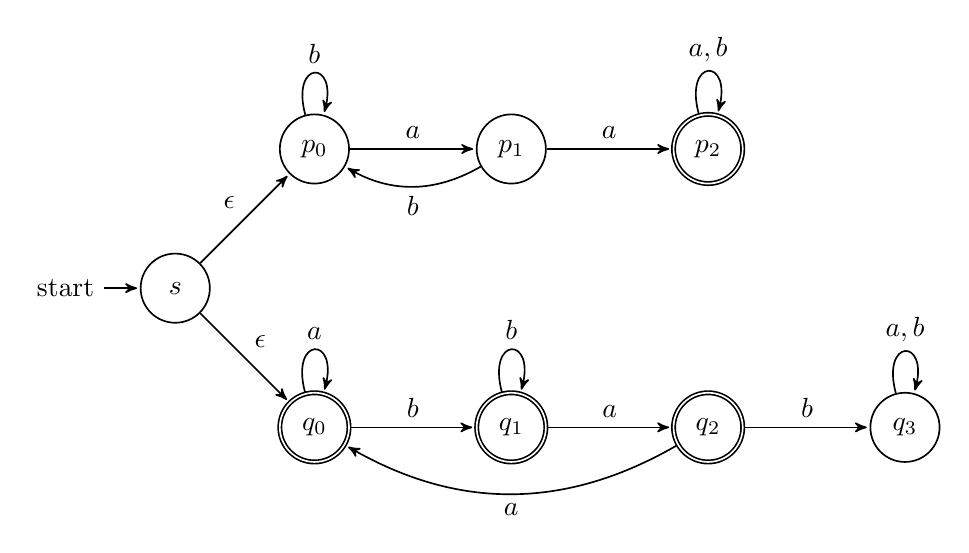
\begin{tikzpicture}[->,>=stealth',shorten >=1pt,auto,node distance=2.5cm,
    semithick]
  \node[initial, state] (qs) {$s$};
  \node[state] [above right of = qs] (q02) {$p_0$};
  \node[state] (q12) [right of=q02] {$p_1$};
  \node[state, accepting] (q22) [right of=q12] {$p_2$};
  \node[state, accepting] (q01) [below right of = qs] {$q_0$};
  \node[state, accepting] (q11) [right of=q01] {$q_1$};
  \node[state, accepting] (q21) [right of=q11] {$q_2$};
  \node[state] (q31) [right of=q21] {$q_3$};
  \path (qs) edge node {$\epsilon$} (q01)
  edge node {$\epsilon$} (q02)
  (q01) edge node {$b$} (q11)
  edge [loop above] node {$a$} (q01)
  (q11) edge [loop above] node {$b$} (q11)
  edge node {$a$} (q21)
  (q21) edge [bend left] node {$a$} (q01)
  edge node {$b$} (q31)
  (q31) edge [loop above] node {$a, b$} (q31)
  (q02) edge node {$a$} (q12)
  edge [loop above] node {$b$} (q02)
  (q12) edge [bend left] node {$b$} (q02)
  edge node {$a$} (q22)
  (q22) edge [loop above] node {$a, b$} (q22);
\end{tikzpicture}
\end{center}

Og vi vet at NFA og DFA er ekvivalente, så vet vi kan kontruere en DFA ut ifra denne NFAen.
Forenkler fortløpende, uten å vise utregning.

\begin{center}
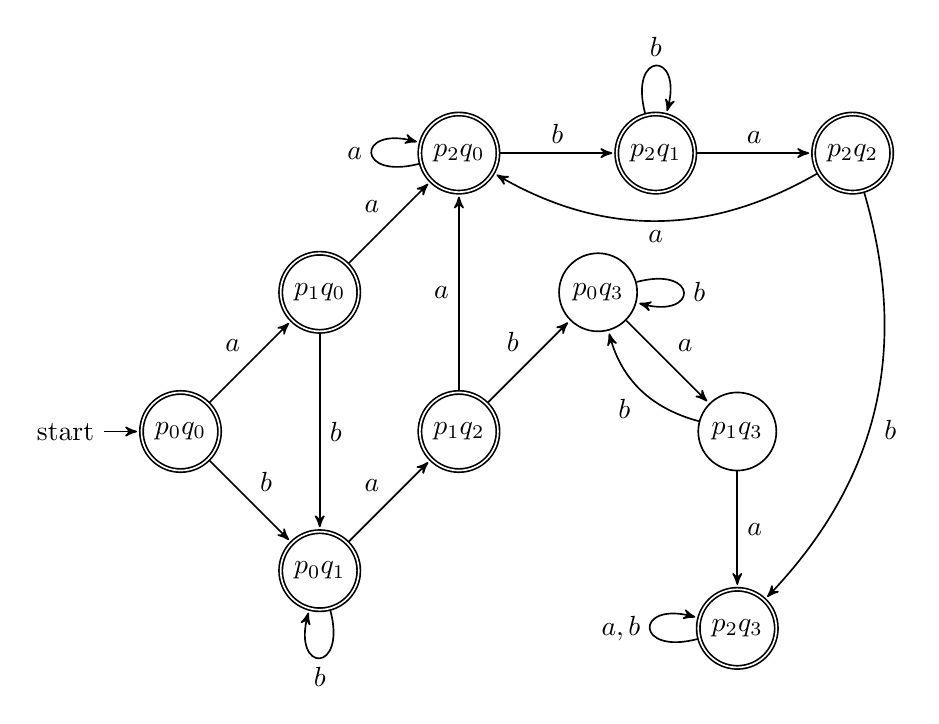
\begin{tikzpicture}[->,>=stealth',shorten >=1pt,auto,node distance=2.5cm,
    semithick]
  \node[state, initial, accepting] (p0q0) {$p_0q_0$};
  \node[state, accepting] (p1q0) [above right of = p0q0]{$p_1q_0$};
  \node[state, accepting] (p0q1) [below right of = p0q0]{$p_0q_1$};
  \node[state, accepting] (p2q0) [above right of = p1q0]{$p_2q_0$};
  \node[state, accepting] (p2q1) [right of = p2q0]{$p_2q_1$};
  \node[state, accepting] (p2q2) [right of = p2q1]{$p_2q_2$};
  \node[state, accepting] (p1q2) [above right of = p0q1]{$p_1q_2$};
  \node[state] (p0q3) [above right of = p1q2]{$p_0q_3$};
  \node[state] (p1q3) [below right of = p0q3]{$p_1q_3$};
  \node[state, accepting] (p2q3) [below of = p1q3]{$p_2q_3$};
  \path (p0q0) edge node {$a$} (p1q0)
  edge node {$b$} (p0q1)
  (p1q0) edge node {$a$} (p2q0)
  edge node {$b$} (p0q1)
  (p2q0) edge [loop left] node {$a$} (p2q0)
  edge node {$b$} (p2q1)
  (p2q1) edge [loop above] node {$b$} (p2q1)
  edge node {$a$} (p2q2)
  (p2q2) edge [bend left] node {$a$} (p2q0)
  edge [bend left] node {$b$} (p2q3)
  (p0q1) edge node {$a$} (p1q2)
  edge [loop below] node {$b$} (p0q1)
  (p1q2) edge node {$a$} (p2q0)
  edge node {$b$} (p0q3)
  (p0q3) edge [loop right] node {$b$} (p0q3)
  edge node {$a$} (p1q3)
  (p1q3) edge [bend left] node {$b$} (p0q3)
  edge node {$a$} (p2q3)
  (p2q3) edge [loop left] node {$a,b$} (p2q3)
  ;
\end{tikzpicture}
\end{center}



\subsection{4.}
$\mathcal{L}_3 = \mathcal{L}_1 \cap \mathcal{L}_2 = \overline{\overline{\mathcal{L}_1} \cup \overline{\mathcal{L}_2}}$

La oss se på $\overline{\mathcal{L}_1} \cup \overline{\mathcal{L}_2}$ først. Ser da at det blir samme framgangsmåte som i 3. men at $\mathcal{L}_1$ og $\mathcal{L}_2$ er invertert.
Og vi får følgende:


\begin{center}
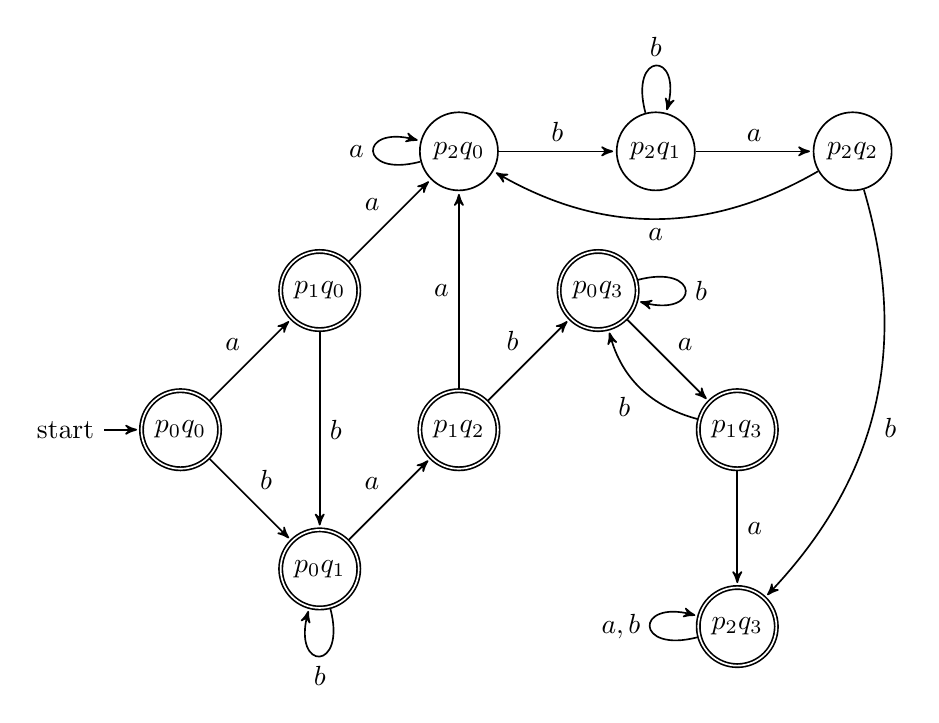
\begin{tikzpicture}[->,>=stealth',shorten >=1pt,auto,node distance=2.5cm,
    semithick]
  \node[state, initial, accepting] (p0q0) {$p_0q_0$};
  \node[state, accepting] (p1q0) [above right of = p0q0]{$p_1q_0$};
  \node[state, accepting] (p0q1) [below right of = p0q0]{$p_0q_1$};
  \node[state] (p2q0) [above right of = p1q0]{$p_2q_0$};
  \node[state] (p2q1) [right of = p2q0]{$p_2q_1$};
  \node[state] (p2q2) [right of = p2q1]{$p_2q_2$};
  \node[state, accepting] (p1q2) [above right of = p0q1]{$p_1q_2$};
  \node[state, accepting] (p0q3) [above right of = p1q2]{$p_0q_3$};
  \node[state, accepting] (p1q3) [below right of = p0q3]{$p_1q_3$};
  \node[state, accepting] (p2q3) [below of = p1q3]{$p_2q_3$};
  \path (p0q0) edge node {$a$} (p1q0)
  edge node {$b$} (p0q1)
  (p1q0) edge node {$a$} (p2q0)
  edge node {$b$} (p0q1)
  (p2q0) edge [loop left] node {$a$} (p2q0)
  edge node {$b$} (p2q1)
  (p2q1) edge [loop above] node {$b$} (p2q1)
  edge node {$a$} (p2q2)
  (p2q2) edge [bend left] node {$a$} (p2q0)
  edge [bend left] node {$b$} (p2q3)
  (p0q1) edge node {$a$} (p1q2)
  edge [loop below] node {$b$} (p0q1)
  (p1q2) edge node {$a$} (p2q0)
  edge node {$b$} (p0q3)
  (p0q3) edge [loop right] node {$b$} (p0q3)
  edge node {$a$} (p1q3)
  (p1q3) edge [bend left] node {$b$} (p0q3)
  edge node {$a$} (p2q3)
  (p2q3) edge [loop left] node {$a,b$} (p2q3)
  ;
\end{tikzpicture}
\end{center}




Inverterer vi så hele DFAen får vi

\begin{center}
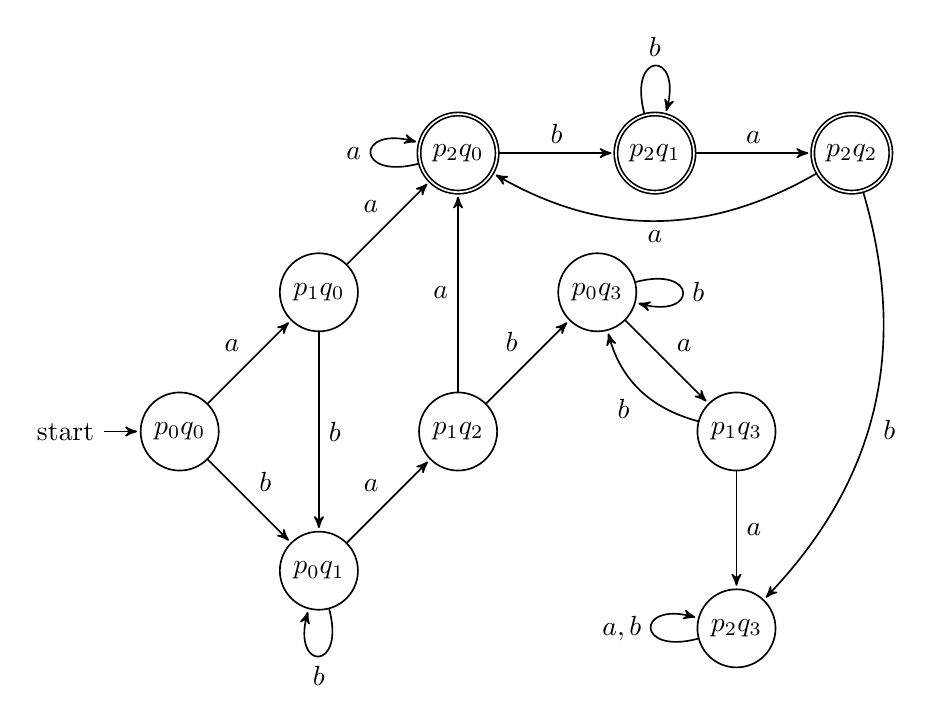
\begin{tikzpicture}[->,>=stealth',shorten >=1pt,auto,node distance=2.5cm,
    semithick]
  \node[state, initial] (p0q0) {$p_0q_0$};
  \node[state] (p1q0) [above right of = p0q0]{$p_1q_0$};
  \node[state] (p0q1) [below right of = p0q0]{$p_0q_1$};
  \node[state, accepting] (p2q0) [above right of = p1q0]{$p_2q_0$};
  \node[state, accepting] (p2q1) [right of = p2q0]{$p_2q_1$};
  \node[state, accepting] (p2q2) [right of = p2q1]{$p_2q_2$};
  \node[state] (p1q2) [above right of = p0q1]{$p_1q_2$};
  \node[state] (p0q3) [above right of = p1q2]{$p_0q_3$};
  \node[state] (p1q3) [below right of = p0q3]{$p_1q_3$};
  \node[state] (p2q3) [below of = p1q3]{$p_2q_3$};
  \path (p0q0) edge node {$a$} (p1q0)
  edge node {$b$} (p0q1)
  (p1q0) edge node {$a$} (p2q0)
  edge node {$b$} (p0q1)
  (p2q0) edge [loop left] node {$a$} (p2q0)
  edge node {$b$} (p2q1)
  (p2q1) edge [loop above] node {$b$} (p2q1)
  edge node {$a$} (p2q2)
  (p2q2) edge [bend left] node {$a$} (p2q0)
  edge [bend left] node {$b$} (p2q3)
  (p0q1) edge node {$a$} (p1q2)
  edge [loop below] node {$b$} (p0q1)
  (p1q2) edge node {$a$} (p2q0)
  edge node {$b$} (p0q3)
  (p0q3) edge [loop right] node {$b$} (p0q3)
  edge node {$a$} (p1q3)
  (p1q3) edge [bend left] node {$b$} (p0q3)
  edge node {$a$} (p2q3)
  (p2q3) edge [loop left] node {$a,b$} (p2q3)
  ;
\end{tikzpicture}
\end{center}

\end{document}
